\documentclass[9pt]{beamer}

\usetheme[progressbar=frametitle]{metropolis}
\usepackage[italian]{babel}

\usepackage{paralist}

\usepackage{appendixnumberbeamer}

\usepackage{amsmath}

\usepackage{booktabs}
\usepackage[scale=2]{ccicons}

\usepackage{pgfplots}
\usepgfplotslibrary{dateplot}

\usepackage{xspace}
\newcommand{\themename}{\textbf{\textsc{metropolis}}\xspace}

\title{TSP con pick up and delivery}
\subtitle{Progetto del corso di Ricerca Operativa}
\date{13 dicembre 2022}
\author{Michele Vaccari - Matricola 121955}
\institute{Università degli studi di Ferrara\\Corso di laurea magistrale in Ingegneria Informatica e dell'Automazione\\AA 2020-2021}

% logo of my university
\titlegraphic{%
  \begin{picture}(0,0)
    \put(305,0){\makebox(0,0)[rt]{
\includegraphics[width=4cm]{../images/logo-unife}}}
  \end{picture}}

\usepackage{minted}
\usepackage{multicol}
\usepackage{multirow}
\usepackage{adjustbox}
\usepackage{graphicx}

\begin{document}

\maketitle

\begin{frame}[allowframebreaks]{Indice}
  \setbeamertemplate{section in toc}[sections numbered]
  \tableofcontents
\end{frame}

\section{Introduzione}

\subsection{Descrizione del problema}
\begin{frame}{\subsecname}

	\metroset{block=fill}
	\begin{block}{Progettino 24 - TSP con pick up and delivery (1 persona)}
		A partire dalla base (nodo $0$ del grafo) un corriere deve soddisfare $n$ richieste di prelievo e consegna di documenti:
		\begin{compactitem}
			\item 	ogni documento è prelevato in un nodo e consegnato in un altro nodo;
			\item ogni nodo è riferito a una singola richiesta, ma nel tragitto tra punto di prelievo e consegna si possono prelevare/consegnare altri documenti.
		\end{compactitem}
		Noto il tempo di percorrenza dei singoli archi, si vuole minimizzare la durata del percorso, con partenza e rientro al deposito.
	\end{block}

\end{frame}

\subsection{Un esempio di istanza}
\begin{frame}{\subsecname}

	\begin{figure}[h]
		\centering
		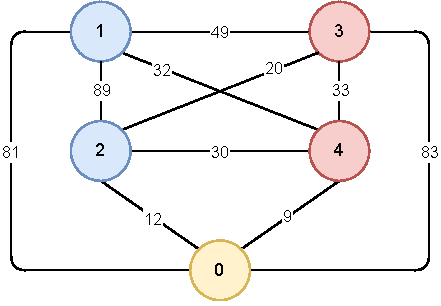
\includegraphics[width=0.6\textwidth]
		{../images/graph-tsppd-with-two-customers}	
		\caption{Istanza con 2 richieste di prelievo e consegna}
	\end{figure}

\end{frame}

\section{Modello matematico per S-TSPPD}
\subsection{Notazione}
\begin{frame}[allowframebreaks]{\subsecname}
	\begin{itemize}
		\item
		Numero di richieste di prelievo e consegna: $n$
		
		\item
		Nodi di pickup: $V_P = \{1, \dots, n\}$
		
		\item
		Nodi di delivery: $V_D = \{n+1, \dots, 2n\}$
		
		\item
		Una richiesta è identificata con la coppia di nodi $(i,n+i)$ e $i$ deve precedere $n+i$ in un percorso ammissibile
		
		\item
		$V$ è definito come l'unione di $V_P$ e $V_D$ con l'aggiunta del nodo di deposito $\{0\}$
		
		\item
		$E_{PD}$ è l'insieme degli archi che connettono $V_P \cup V_D$
	
		\item
		$E$ è l'unione di $E_{PD}$ con tutti gli archi ammissibili che collegano il nodo di deposito
		
		\item
		Il grafo $G=(V,E)$ comprende tutti i nodi e gli archi necessari per descrivere il S-TSPPD (il grafo è completo)
		\[ V=\{0\} \cup V_P \cup V_D \]
		\[ E = \{ (0,i) | i \in V_P \} \cup \{ (0,i) | i \in V_D \} \cup E_{PD} \]
		
		L'insieme degli archi $E$ è definito in modo tale da includere solo archi ammissibili.
		In altre parole, non è possibile che un percorso TSPPD inizi con una consegna o finisca con un prelievo.
		
		\item
		Ogni arco $(i,j) \in E$ è uguale all'arco $(j, i)$

		\item
		Ogni arco ha gli stessi costi e variabili

		\item
		$c_{ij}$ è un costo non negativo per ogni arco $(i,j) \in E$

		\item
		$x_{ij} \in \{ 0, 1 \}$ è una variabile decisionale binaria per ogni $(i, j) \in E$ con il valore $x_{ij} = 1$ se l'arco $(i, j)$ è in una soluzione e $0$ altrimenti

		\item
		$\delta(S) = \{ (i, j) \in E | i \in S, j \notin S$ è il taglio contenente gli archi che collegano $S \subset V$ e $S^* \subset V$ 

		\item
		Per qualsiasi nodo $i \in V, \delta(i) = \delta( \{ i \})$
	\end{itemize}
\end{frame}

\subsection{Modello matematico}
\begin{frame}{\subsecname}

     	\[ min{ \sum_{(i,j) \in E} c_i x_{ij}} \]
	tale che
	\begin{enumerate}
		\item
		\label{stsppd-c1}
		$x_0 = 1$

		\item
		\label{stsppd-c2}
		$x(\delta(i)) = 2 \quad \forall i \in V$

		\item
		\label{stsppd-c3}
		$x(\delta(i)) \geq 2 \quad \forall S \subset V$
	
		\item
		\label{stsppd-c4}
		$x(\delta(i)) \geq 4 \quad \forall S \subset V, \{0, n+i\} \subset S, \{0,i\} \subset V \setminus S$

		\item
		$x_{ij} \in \{0,1\} \quad (i,j) \in E$
	\end{enumerate}
	
	\footnotesize
	Il vincolo \ref{stsppd-c1} richiede che l'arco che collega il nodo di deposito faccia parte di qualsiasi soluzione ammissibile. \\
	Il vincolo \ref{stsppd-c2} richiede che ogni nodo entri ed esca in tutti i percorsi ammissibili, ma di per sé lascia aperta la possibilità di sotto-tour, formando una rappresentazione completa del TSP. \\
	Il vincolo \ref{stsppd-c3} consente di eliminare i sotto-tour, formando una rappresentazione completa del TSP. \\
	Il vincolo \ref{stsppd-c4} richiede che i ritiri avvengano prima delle rispettive consegne

\end{frame}

\section{Modello matematico per A-TSPPD}
\subsection{Notazione}
\begin{frame}[allowframebreaks]{\subsecname}
	\begin{itemize}
		\item
		Numero di richieste di prelievo e consegna: $n$
		
		\item
		Nodi di pickup: $N_P = \{1, \dots, n\}$
		
		\item
		Nodi di delivery: $N_D = \{n+1, \dots, 2n\}$
		
		\item
		Una richiesta è identificata con la coppia di nodi $(i,n+i)$ e $i$ deve precedere $n+i$ in un percorso ammissibile
		
		\item
		$N$ è definito come l'unione di $N_P$ e $N_D$ con l'aggiunta del nodo di deposito $\{0\}$
		
		\item
		$A_{PD}$ è l'insieme degli archi \emph{orientati} che connettono $N_P \cup N_D$
	
		\item
		$A$ è l'unione di $A_{PD}$ con tutti gli archi \emph{orientati} ammissibili che collegano il nodo di deposito
		
		\item
		Il grafo $G=(N,A)$ comprende tutti i nodi e gli archi necessari per descrivere il A-TSPPD (il grafo è completo)
		\begin{equation*}
			\begin{aligned}
			N= & \{0\} \cup N_P \cup N_D \\
			A = & \{ (0,i) | i \in N_P \} \\
			& \cup \{ (i,0) | i \in N_D \} \\
			& \cup \{ (i,j) | i \in N_P , j \in ( N_P \cup N_D ) \setminus \{ i \} \} \\
			& \cup \{ ( n + i, j) | i \in N_P , j \in (N_P \cup N_D ) \setminus \{ i , n + i \} \}
			\end{aligned}
		\end{equation*}
		
		L'insieme degli archi $A$ è definito in modo tale da includere solo archi ammissibili.
		In altre parole, non è possibile che un percorso TSPPD inizi con una consegna o finisca con un prelievo.

		\item
		$c_{ij}$ è un costo non negativo per ogni arco $(i,j) \in A$

		\item
		$x_{ij} \in \{ 0, 1 \}$ è una variabile decisionale binaria per ogni $(i, j) \in A$ con il valore $x_{ij} = 1$ se l'arco $(i, j)$ è in una soluzione e $0$ altrimenti

		\item
		$\delta(S) = \{ (i, j) \in A | i \in S, j \notin S$ è il taglio contenente gli archi che collegano $S \subset N$ e $S^* \subset N$ 

		\item
		Per qualsiasi nodo $i \in N, \delta(i) = \delta( \{ i \})$
	\end{itemize}
\end{frame}

\subsection{Modello matematico}
\begin{frame}{\subsecname}

     	\[ min{ \sum_{(i,j) \in A} c_i x_{ij}} \]
	tale che
	\begin{enumerate}
		\item
		\label{atsppd-c1}
		$\sum_{(i,j) \in A} x_{ij} = 1 \quad \forall i \in N$

		\item
		\label{atsppd-c2}
		$\sum_{(i,j) \in A} x_{ij} = 1 \quad \forall j \in N$

		\item
		\label{atsppd-c3}
		$x(\delta(S)) \geq 1 \quad \forall S \subset N$
	
		\item
		\label{atsppd-c4}
		$x(\delta(i)) \geq 4 \quad \forall S \subset N, \{0, n+i\} \subset S, \{0,i\} \subset N \setminus S$

		\item
		$x_{ij} \in \{0,1\} \quad (i,j) \in A$
	\end{enumerate}
	
	\footnotesize
	I vincoli \ref{atsppd-c1} e \ref{atsppd-c2} richiedono che ogni nodo preceda e segua direttamente un altro nodo. \\
	Il vincolo \ref{atsppd-c3} consente di eliminare i sotto-tour, formando una rappresentazione completa del TSP. \\
	Il vincolo \ref{atsppd-c4} richiede che i ritiri avvengano prima delle rispettive consegne (è uguale al vincolo \ref{stsppd-c4} del S-TSPPD)

\end{frame}

\begin{frame}{Alcune considerazioni sul problema}
	
	\begin{itemize}
	
		\item
		Di fatto il TSPPD è un TSP con in più i vincoli di precedenza.

		\item
		Sia S-TSPPD che A-TSPPD sono formulazioni che pongono dei problemi per il gran numero di vincoli

		\item
		Un'istanza S-TSP con $n$ coppie ha \( \#TSP = \frac{1}{2} (2n -1)!\) soluzioni distinte \cite{lin1965computer}, mentre un TSPPD della stessa dimensione ha \(\#TSPPD(n) = \frac{2n!}{2^n}\) \cite{ruland1997pickup}
		
		\item
		La dimensione dell'insieme ammissibile del TSPPD cresce più lentamente rispetto al numero di coppie di nodi rispetto a quella del TSP

		\item
		Ovviamente, l'insieme delle soluzioni ammissibili del TSPPD è un sottoinsieme delle soluzioni fattibili del TSP
		
		\item
		Se si ammettono solo coppie di nodi di ritiro e consegna nel percorso con relazioni di precedenza, la dimensione dell'insieme fattibile del TSP si riduce di \( \frac{1}{2^{n-1}!} \) \cite{ruland1997pickup}
	\end{itemize}

\end{frame}

\subsection{Soluzioni ammissibili per l'istanza d'esempio}
\begin{frame}{\subsecname}

	\begin{figure}[h]
		\centering
		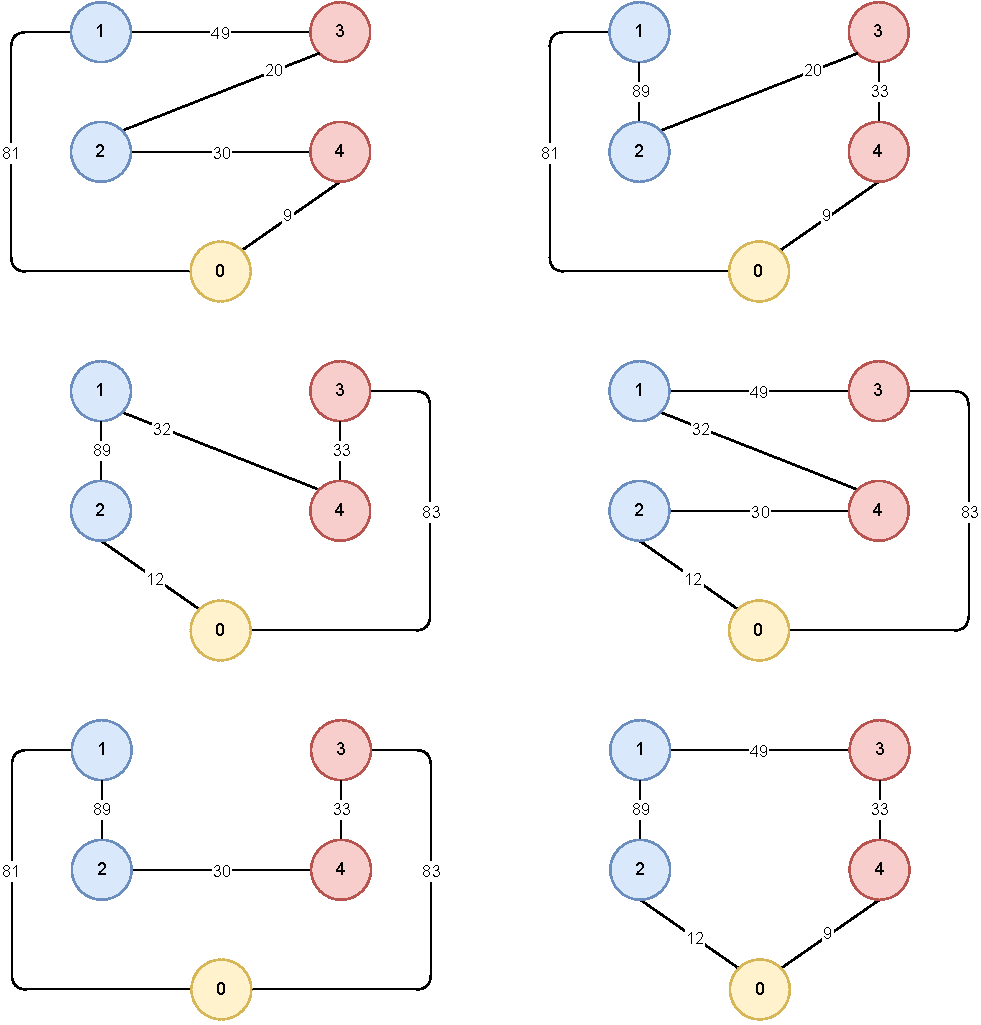
\includegraphics[width=0.6\textwidth]
		{../images/graph-all-solutions-tsppd-with-two-customers}	
		\caption{Soluzioni ammissibili per l'istanza con 2 richieste di prelievo e consegna}
	\end{figure}

\end{frame}

\section{Progetto}

\subsection{Organizzazione}
\begin{frame}[allowframebreaks]{\subsecname}

	\textbf{Strumenti utilizzati}
	\begin{itemize}
		\item
		Linguaggio Python 3.10 con le seguenti librerie:
		\begin{itemize}
			\item
			Click
			\item
			Numpy
			\item
			Pytest
			\item
			Openpyxl
			\item
			Stopwatch
		\end{itemize}
		\item
		Visual Studio Code come editor di testo
		\item
		Git per il versionamento del codice
	\end{itemize}

\framebreak

	\textbf{Arichitettura} \\
	L’applicazione è formata da 3 componenti:
	\begin{itemize}
		\item
		\textbf{problem:} è il package che contiene le entità utilizzate per modellare il problema e un generatore di istanze casuali
		\item
		\textbf{solver:} è il package che contiene gli algoritmi implementati. Utilizza le entità definite nel package problem
		\item
		\textbf{cli:} è una Command Line Interface che consente di generare istanze del problema e testare i vari algoritmi
	\end{itemize}

	\textbf{Repository GitHub} \href{https://github.com/michele-vaccari/TSP-con-pick-up-and-delivery}{https://github.com/michele-vaccari/TSP-con-pick-up-and-delivery}

\end{frame}

\subsection{Benchmark}
\begin{frame}{\subsecname}

	\textbf{Automazione} \\
	L'esecuzione e la raccolta dei dati durante i benchmark è stata automatizzata sempre utilizzando il linguaggio Python. Si è utilizzata la libreria Openpyxl in modo tale che i dati vengano collezionati in modo ordinato su fogli di calcolo.

	\textbf{Esecuzione} \\
	I benchmark sono stati eseguiti su un PC con:
	\begin{itemize}
		\item
		\textbf{Sistema operativo:} Windows 10
		\item
		\textbf{Processore:} Intel Core i5-4570 CPU  3.20 GHz
		\item
		\textbf{RAM:} 16.0 GB
	\end{itemize}
	Il tempo di esecuzione complessivo dei benchmark è stato di circa $10$ giorni. Nel dettaglio: $346399.9\;secondi \rightarrow 5773.332\;minuti \rightarrow 240.5555\;ore \rightarrow 10.02315\;giorni$

\end{frame}

\subsection{Generatore di istanze}
\begin{frame}[fragile]{\subsecname}

	È possible generare un istanza del problema nel seguente modo:
	\begin{itemize}
		\item
		\textbf{Istanza asimmetrica} \\
		\mintinline[breaklines]{bash}{python tsppdcli.py generate-instance --requests 2 --weights-random --output-instance-path 2-request-weights-random.jsonn}
		\item
		\textbf{Istanza simmestrica} \\
		\mintinline[breaklines]{bash}{python tsppdcli.py generate-instance --requests 2 --weights-as-euclidean-distance --output-instance-path 2-request-weights-euclidean-distance.json}
	\end{itemize}

	\textbf{Esempio di istanza} \\
	\href{https://github.com/michele-vaccari/TSP-con-pick-up-and-delivery/blob/main/src/instances/2-request.json}{https://github.com/michele-vaccari/TSP-con-pick-up-and-delivery/blob/main/src/instances/2-request.json}

\end{frame}

\section{Algoritmi esatti}

\subsection{Brute force enumerator}
\begin{frame}[allowframebreaks]{\subsecname}

	\textbf{Descrizione dell’algoritmo} \\
	Vediamo il codice dell’algoritmo Brute force enumerator:
	\href{https://github.com/michele-vaccari/TSP-con-pick-up-and-delivery/blob/main/src/tsppd/solver/bruteForceEnumerator.py}{https://github.com/michele-vaccari/TSP-con-pick-up-and-delivery/blob/main/src/tsppd/solver/bruteForceEnumerator.py}

	\textbf{Esempio}
	\begin{figure}[h]
	\centering
	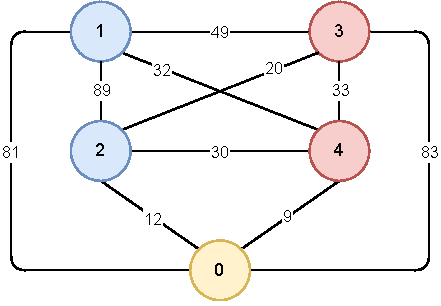
\includegraphics[width=0.4\textwidth]
	{../images/graph-tsppd-with-two-customers}	
	\caption{Istanza iniziale}
	\end{figure}

\framebreak

	\textbf{Esecuzione}
      	\begin{figure}[h]
	\centering
	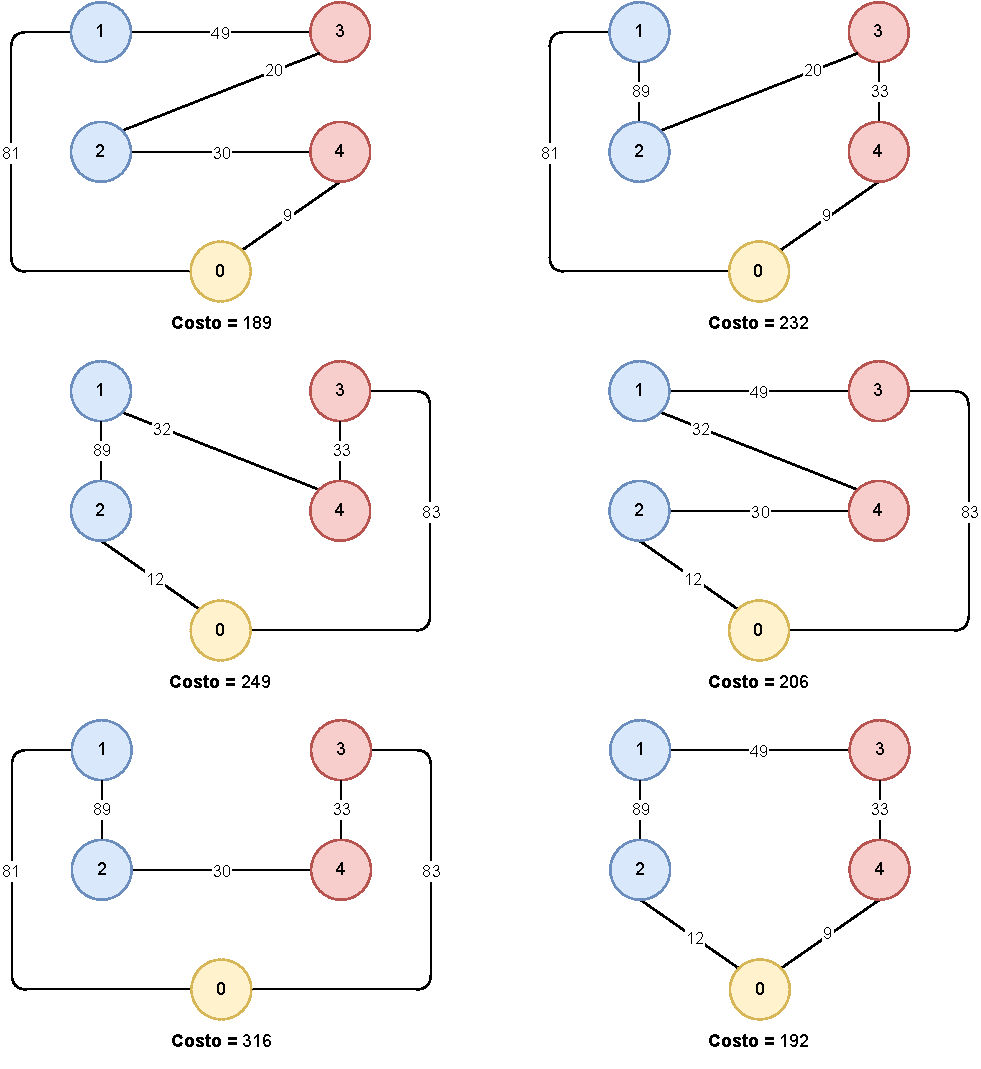
\includegraphics[width=0.45\textwidth]
	{../images/graph-all-solutions-with-cost-tsppd-with-two-customers}	
	\caption{Soluzioni esplorate}
	\end{figure}

\framebreak

	\textbf{Performance nel tempo}
      	\begin{figure}[h]
	\centering
	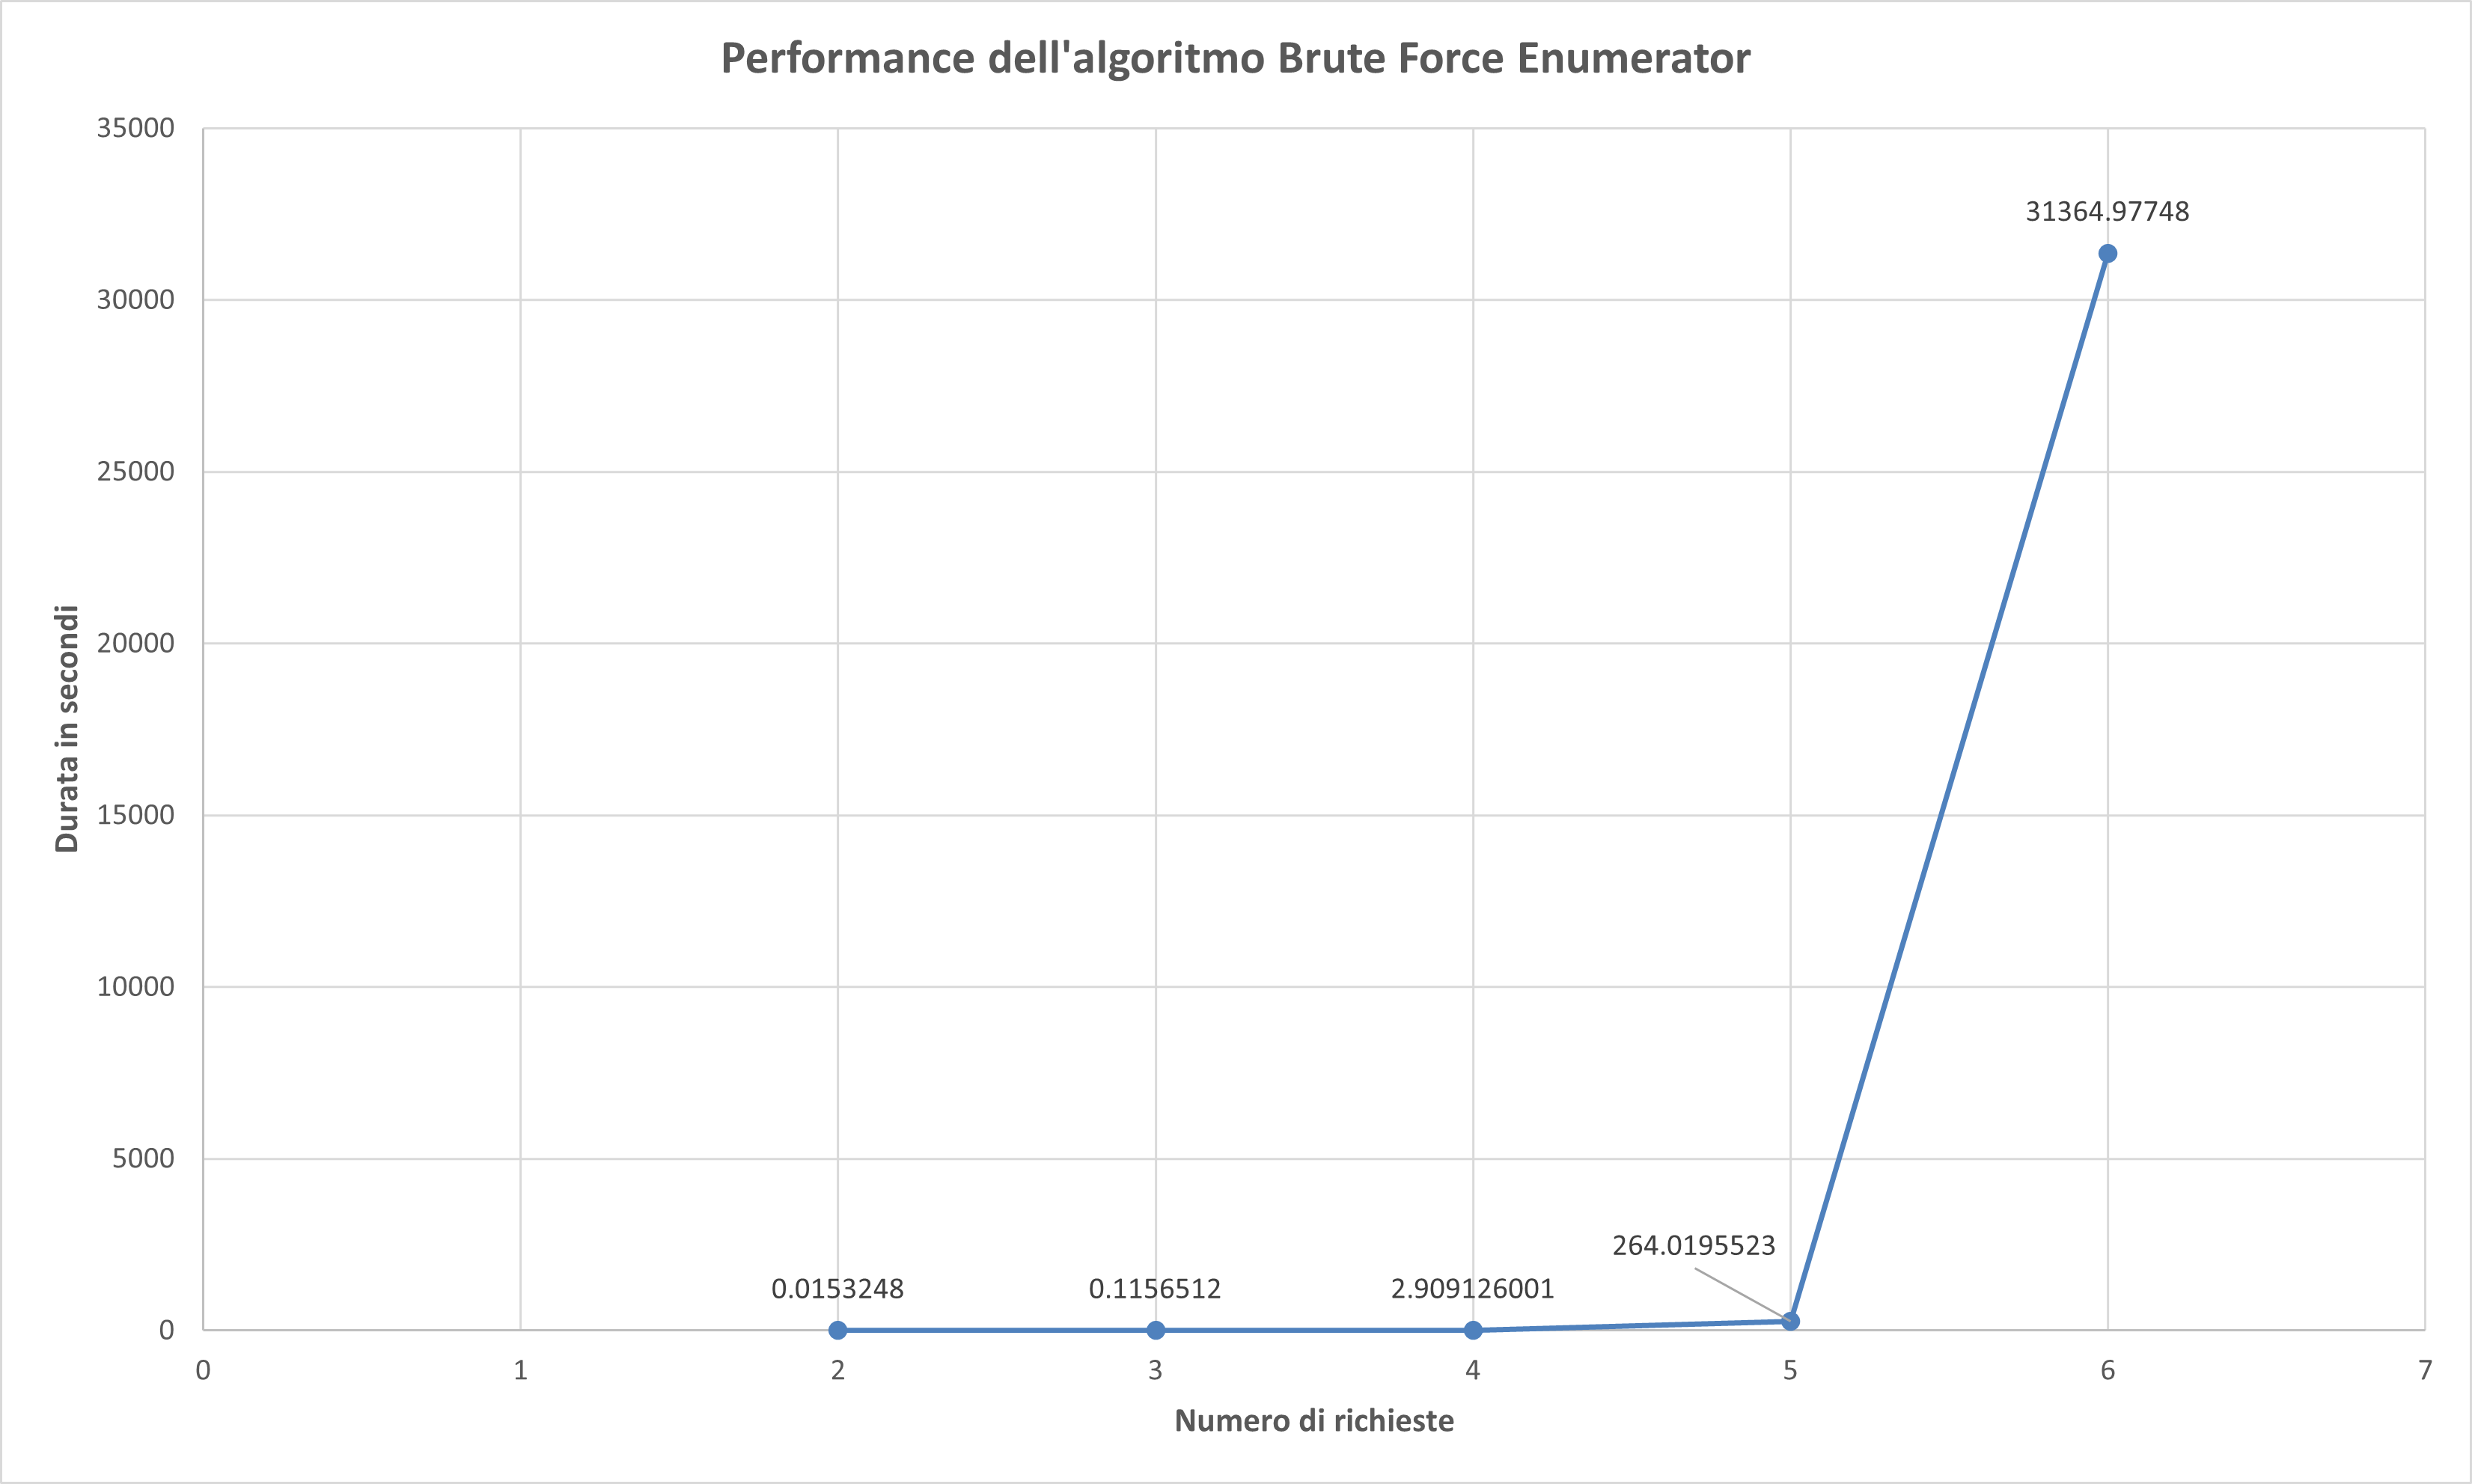
\includegraphics[width=\textwidth]
	{../charts/01 Performance dell'algoritmo Brute Force Enumerator}
	\end{figure}

\end{frame}

\subsection{O’Neil -- Hoffman enumerator}
\begin{frame}[allowframebreaks, fragile]{\subsecname}

	\begin{columns}[T,onlytextwidth]
		\column{0.5\textwidth}
		\begin{minted}[fontsize=\tiny, escapeinside=;;, tabsize=2]{c}
function Initialize()
	for all ;$i \in nodes$; do
		;$arcs(i) \leftarrow ordered \{j | j \in nodes \setminus \{ 0 \} , j \neq i\}$;
	;$tour \leftarrow (0)$;
	;$best \leftarrow \emptyset$;

function Enumerate()
	;$n_1 \leftarrow last\,node\,in\,tour$;
	for all ;$n_2 \in arcs(current)$; do
		if ;$n_2 \in tour$;
			continue
		else if ;$cost(tour) + cost(n_1, n_2) \geq cost(best)$;
			continue
		else if ;$n_2 \in N_D$; and ;$pickup(n_2) \notin tour$;
			continue

	;$tour \leftarrow tour + next$;
	if ;$|tour| \geq n - 1$; then
		;$c \leftarrow cost(tour) + cost(n_2, 0)$;
		if ;$best = \emptyset$; or ;$c < cost(best)$;
			;$best \leftarrow tour + 0$;
	else
		Enumerate()

	;$tour \leftarrow tour - next$;

Initialize()
Enumerate()
		\end{minted}
		\column{0.5\textwidth}
		
		{\scriptsize
		\textbf{Descrizione dell’algoritmo} \\

		L'algoritmo O’Neil -- Hoffman \cite{o2018exact} utilizza una funzione ricorsiva per cercare l'insieme ammissibile dei percorsi TSPPD, tenendo traccia della migliore soluzione scoperta in ogni punto dell'albero di ricerca.

		L'algoritmo mantiene un nodo corrente e un percorso parziale che inizia con $0$ (nodo deposito).

		Ogni ricorsione ripercorre gli archi a partire dal nodo corrente e aggiunge ogni arco ammissibile al tour individualmente prima della ricorsione. Se il costo aggiunto da un arco fa sì che il costo di un percorso parziale sia superiore a quello del tour migliore conosciuto, quell'arco viene ignorato e la sua sezione dell'albero di ricerca viene effettivamente esplorata. Se un percorso completo migliora la soluzione migliore conosciuta, viene memorizzato come nuovo ottimo candidato.

		La chiave della ricerca efficace e della scoperta precoce di buone soluzioni è la tecnica di ordinamento degli archi. Durante l'inizializzazione, ad ogni nodo viene assegnato un vettore ordinato di nodi successivi. Come funzione di ordinamento utilizziamo il costo ascendente dell'arco, ma altri possono essere facilmente incorporati.

		I nodi che non sono fattibili per il percorso parziale corrente vengono saltati.

		}
	
	  \end{columns}

\framebreak

	\textbf{Codice} \\
	\href{https://github.com/michele-vaccari/TSP-con-pick-up-and-delivery/blob/main/src/tsppd/solver/oneilHoffmanEnumerator.py}{https://github.com/michele-vaccari/TSP-con-pick-up-and-delivery/blob/main/src/tsppd/solver/oneilHoffmanEnumerator.py}

	\textbf{Esempio}
	\begin{figure}[h]
	\centering
	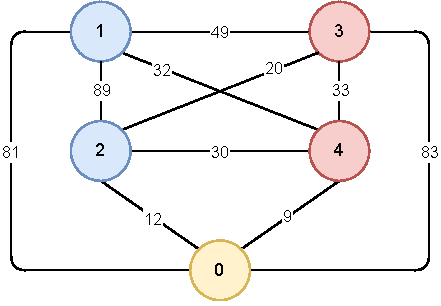
\includegraphics[width=0.5\textwidth]
	{../images/graph-tsppd-with-two-customers}	
	\caption{Istanza iniziale}
	\end{figure}

	\textbf{Esecuzione}
      	\begin{figure}[h]
	\centering
	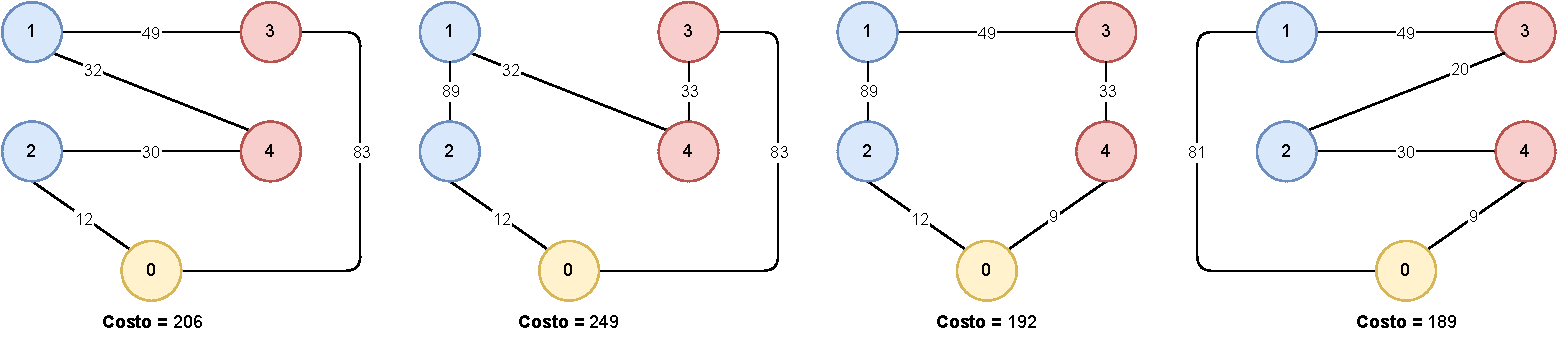
\includegraphics[width=\textwidth]
	{../images/graph-oneil-hoffman-solutions-tsppd-with-two-customers}	
	\caption{Soluzioni esplorate}
	\end{figure}

\framebreak

	\textbf{Performance nel tempo}
      	\begin{figure}[h]
	\centering
	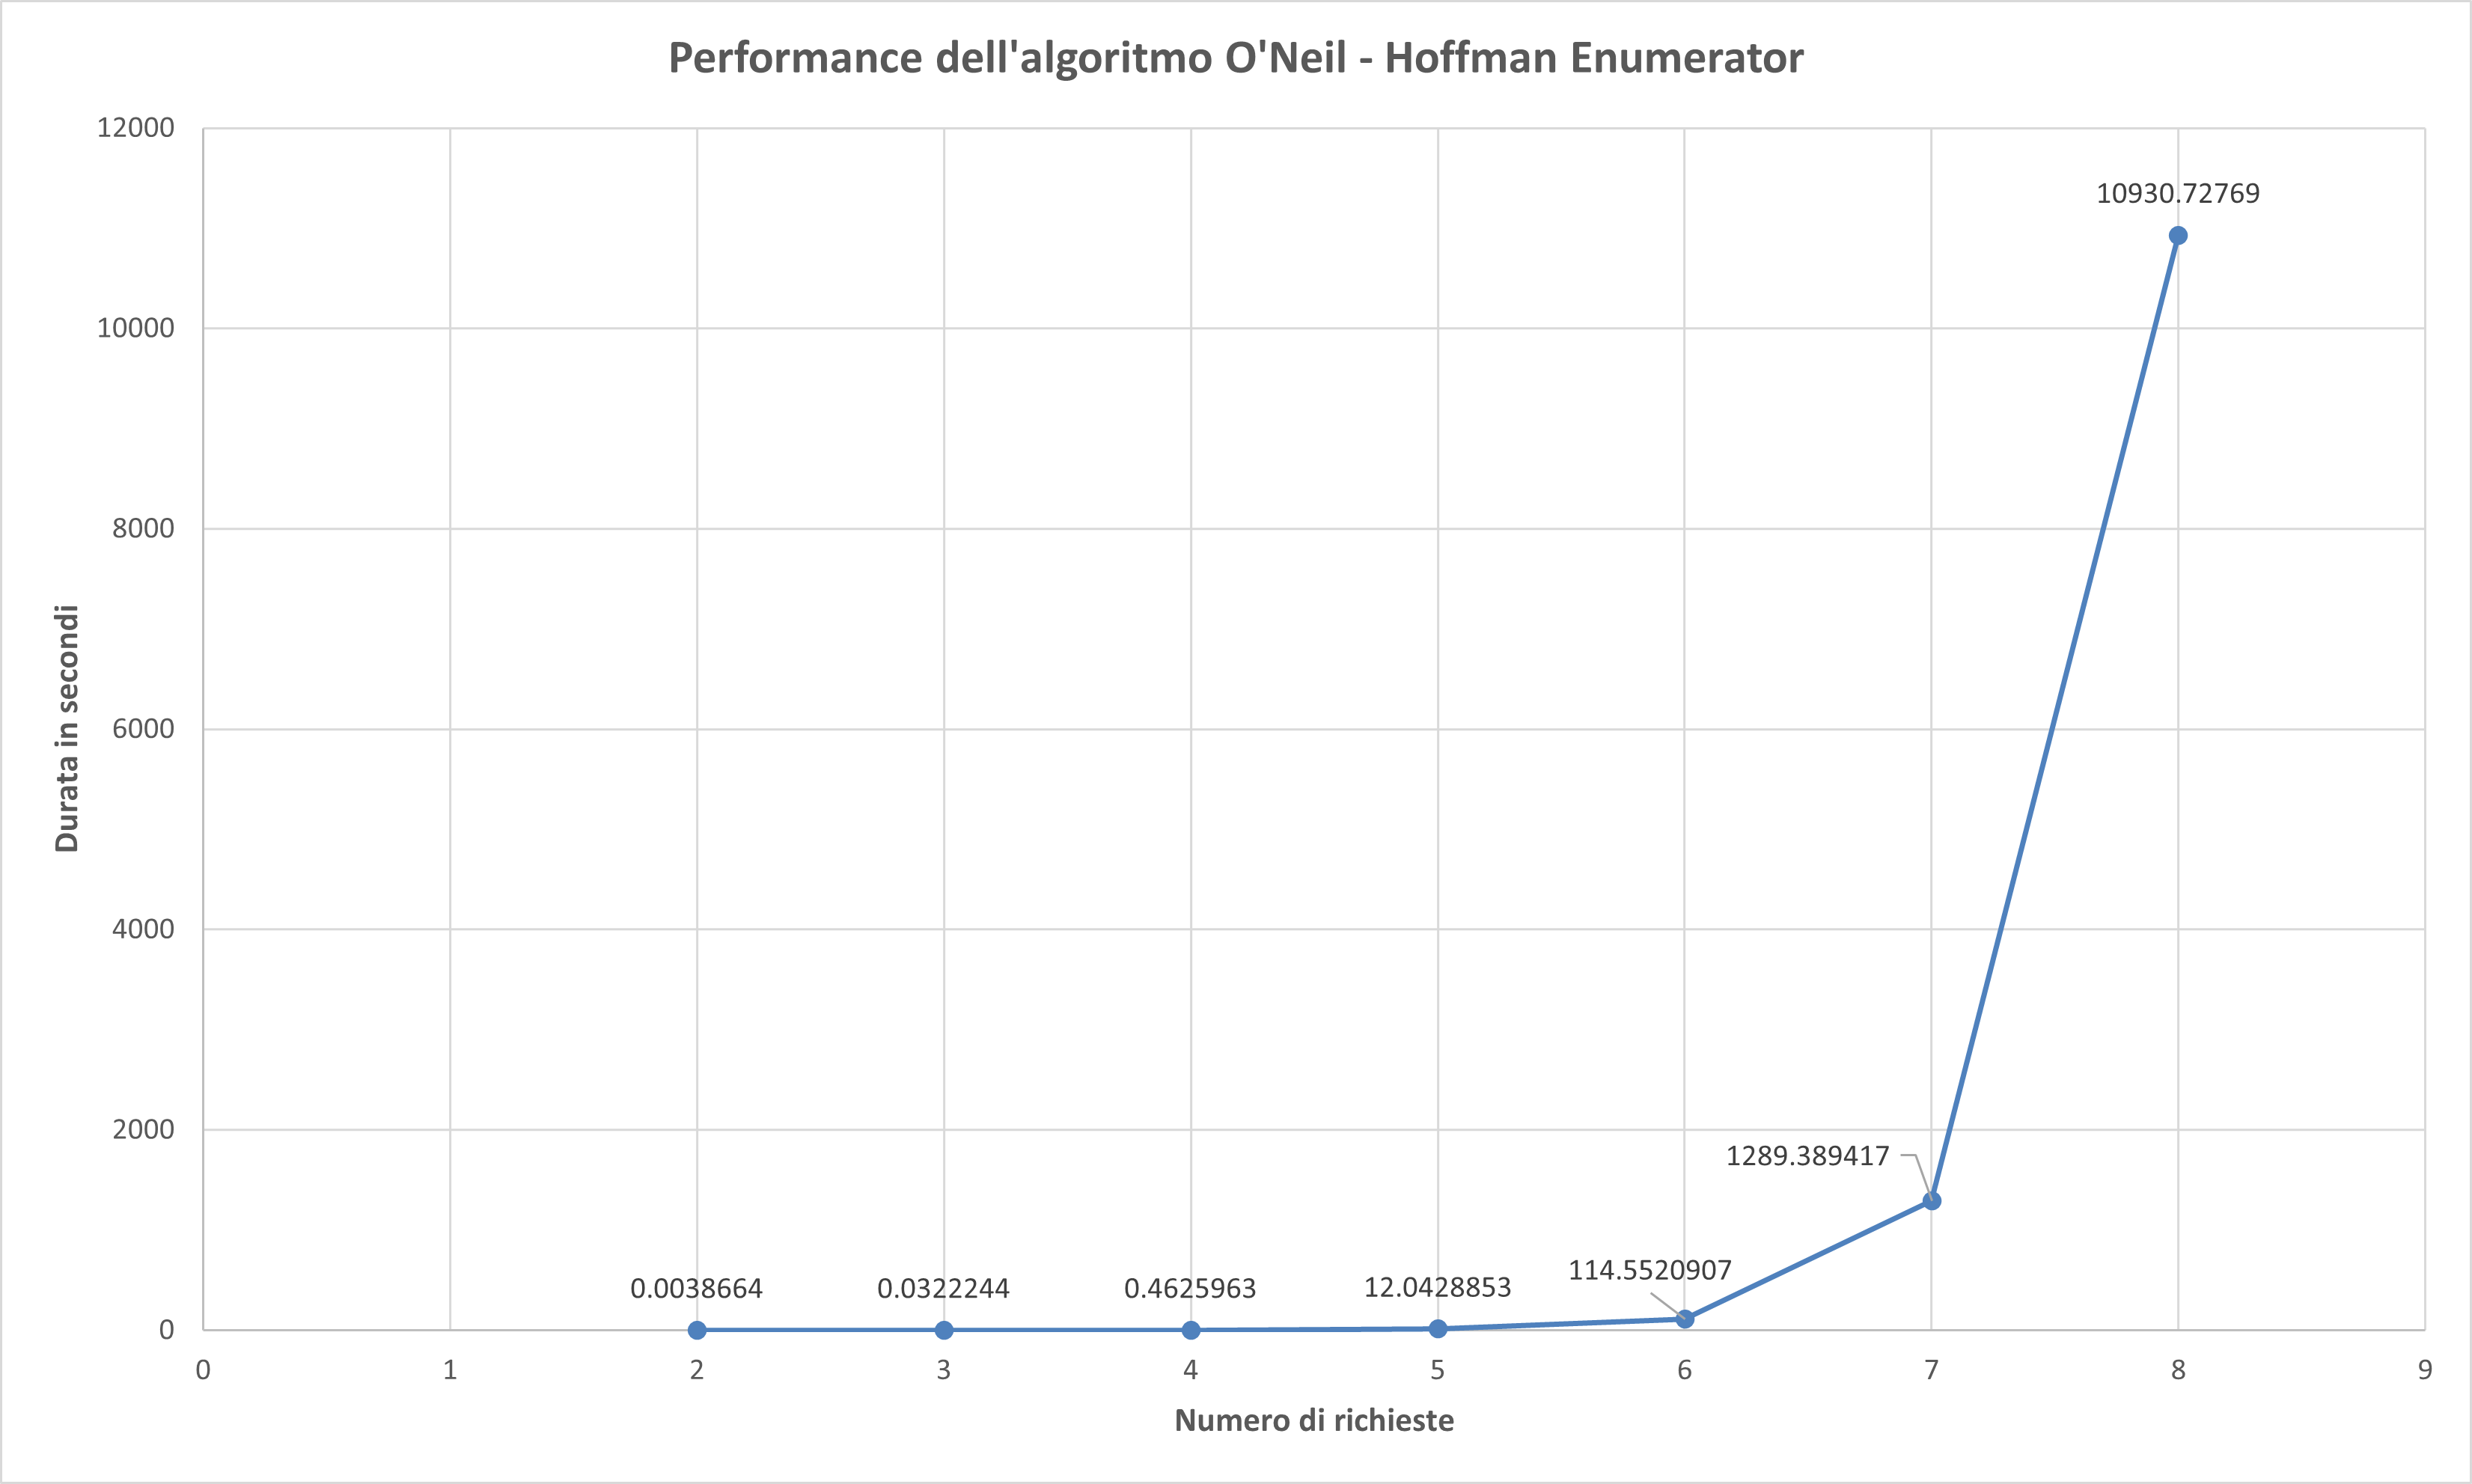
\includegraphics[width=\textwidth]
	{../charts/02 Performance dell'algoritmo O'Neil - Hoffman Enumerator}
	\end{figure}

\end{frame}


\subsection{Confronto}
\begin{frame}[allowframebreaks]{\subsecname}

	\textbf{Performance nel tempo}
      	\begin{figure}[h]
	\centering
	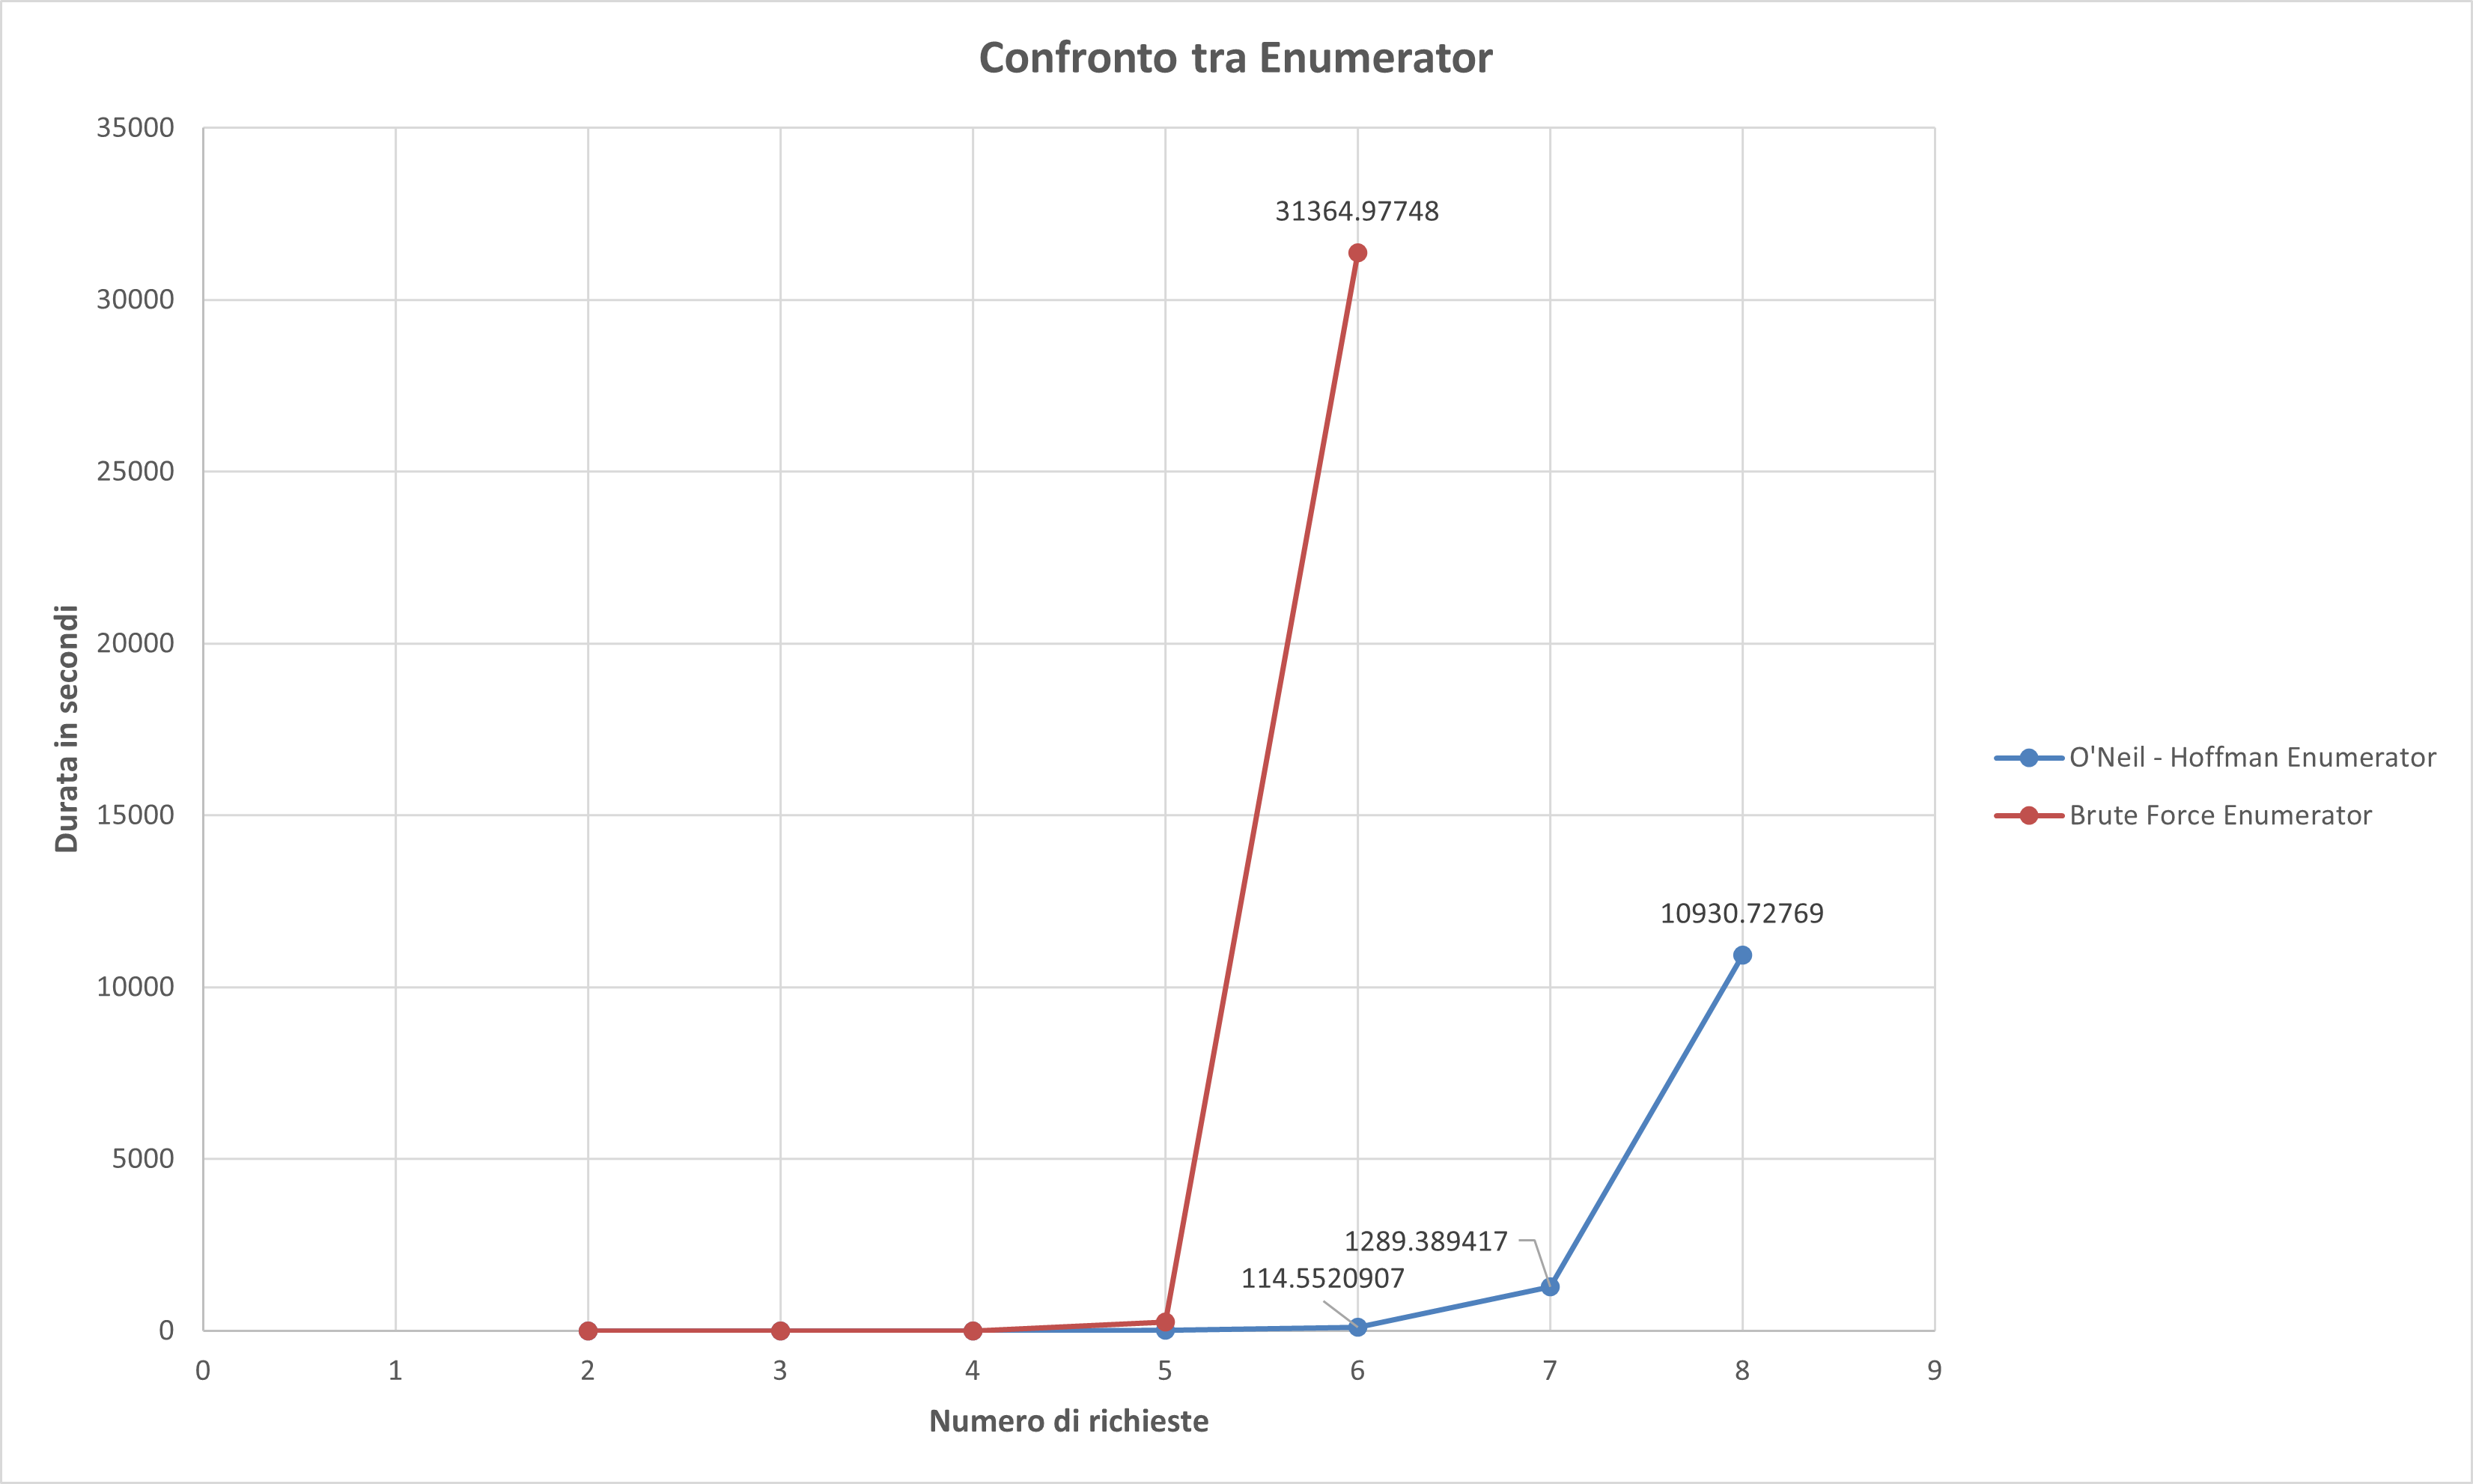
\includegraphics[width=\textwidth]
	{../charts/03 Confronto tra Enumerator}
	\end{figure}

\framebreak

	\textbf{Soluzioni ammissibili esplorate} \\
	I due algoritmi differiscono, oltre che per il tempo di esecuzione anche per il numero di soluzioni ammissibili esplorate

	\begin{table}[h!]
		\centering
		\begin{adjustbox}{max width=\textwidth}
			\begin{tabular}{c c c c c}
				\toprule
				\multirow{2}*{Numero di richieste} & \multicolumn{2}{c}{Brute Force Enumerator} & \multicolumn{2}{c}{O'Neil - Hoffman Enumerator}\\
				& Durata (in secondi) & Soluzioni ammissibili esplorate & Durata (in secondi) & Soluzioni ammissibili esplorate \\
				\midrule
				2 & 0.0153248 & 6 & 0.0038664 & 3 \\
				3 & 0.1156512 & 90 & 0.0322244 & 10 \\
				4 & 2.909126001 & 2520 & 0.4625963 & 3 \\
				5 & 264.0195523 & 113400 & 12.0428853 & 23 \\
				6 & 31364.97748 & 7484400 & 114.5520907 & 115 \\
				7 & N.A. & N.A. & 1289.389417 & 191 \\
				8 & N.A. & N.A. & 10930.72769 & 24 \\
				\bottomrule
			\end{tabular}
		\end{adjustbox}
		\caption{Numero di soluzioni ammissibili esplorate dagli enumeratori}
	\end{table}

	L’enumerazione può essere una tecnica valida per risolvere piccoli TSPPD. Se guidata da alcune informazioni sul problema, l'enumerazione può essere in grado di scoprire rapidamente percorsi validi senza l'onere della formulazione del modello.

\end{frame}


%\begin{frame}[allowframebreaks]{Considerazioni sul problerma}
%	Questo problema di ottimizzazione è NP-hard, poiché coincide con il TSP quando la capacità del veicolo è sufficientemente grande.
%	Anche il problema di verificare se esiste una soluzione ammissibile è un problema fortemente NP-hard, dato che il problema della 3-partizione è un caso particolare (si veda [10] per i dettagli).
%\end{frame}

%\begin{frame}[allowframebreaks]{Interpretazione dei risultati del modello teorico nel problema reale}
%\end{frame}

\begin{frame}{Bibliografia}

	\bibliography{bibliografia.bib}
	\bibliographystyle{abbrv}

\end{frame}

\begin{frame}[standout]
Grazie per l'attenzione
\end{frame}

\end{document}